\documentclass{article}

\usepackage[utf8]{inputenc}
\usepackage{CJK}
\usepackage{tikz}
\usepackage{svg}
\usepackage{graphicx}
\usetikzlibrary{shapes,arrows}

\begin{document}
\begin{CJK}{UTF8}{gbsn}
The purpose of dot2tex is to give graphs generated by Graphviz a more LaTeX friendly look and feel. This is accomplished by converting xdot output from Graphviz to a series of PSTricks or PGF/TikZ commands. This approach allows:你好 wewee

\begin{figure}[h]
    \centering
    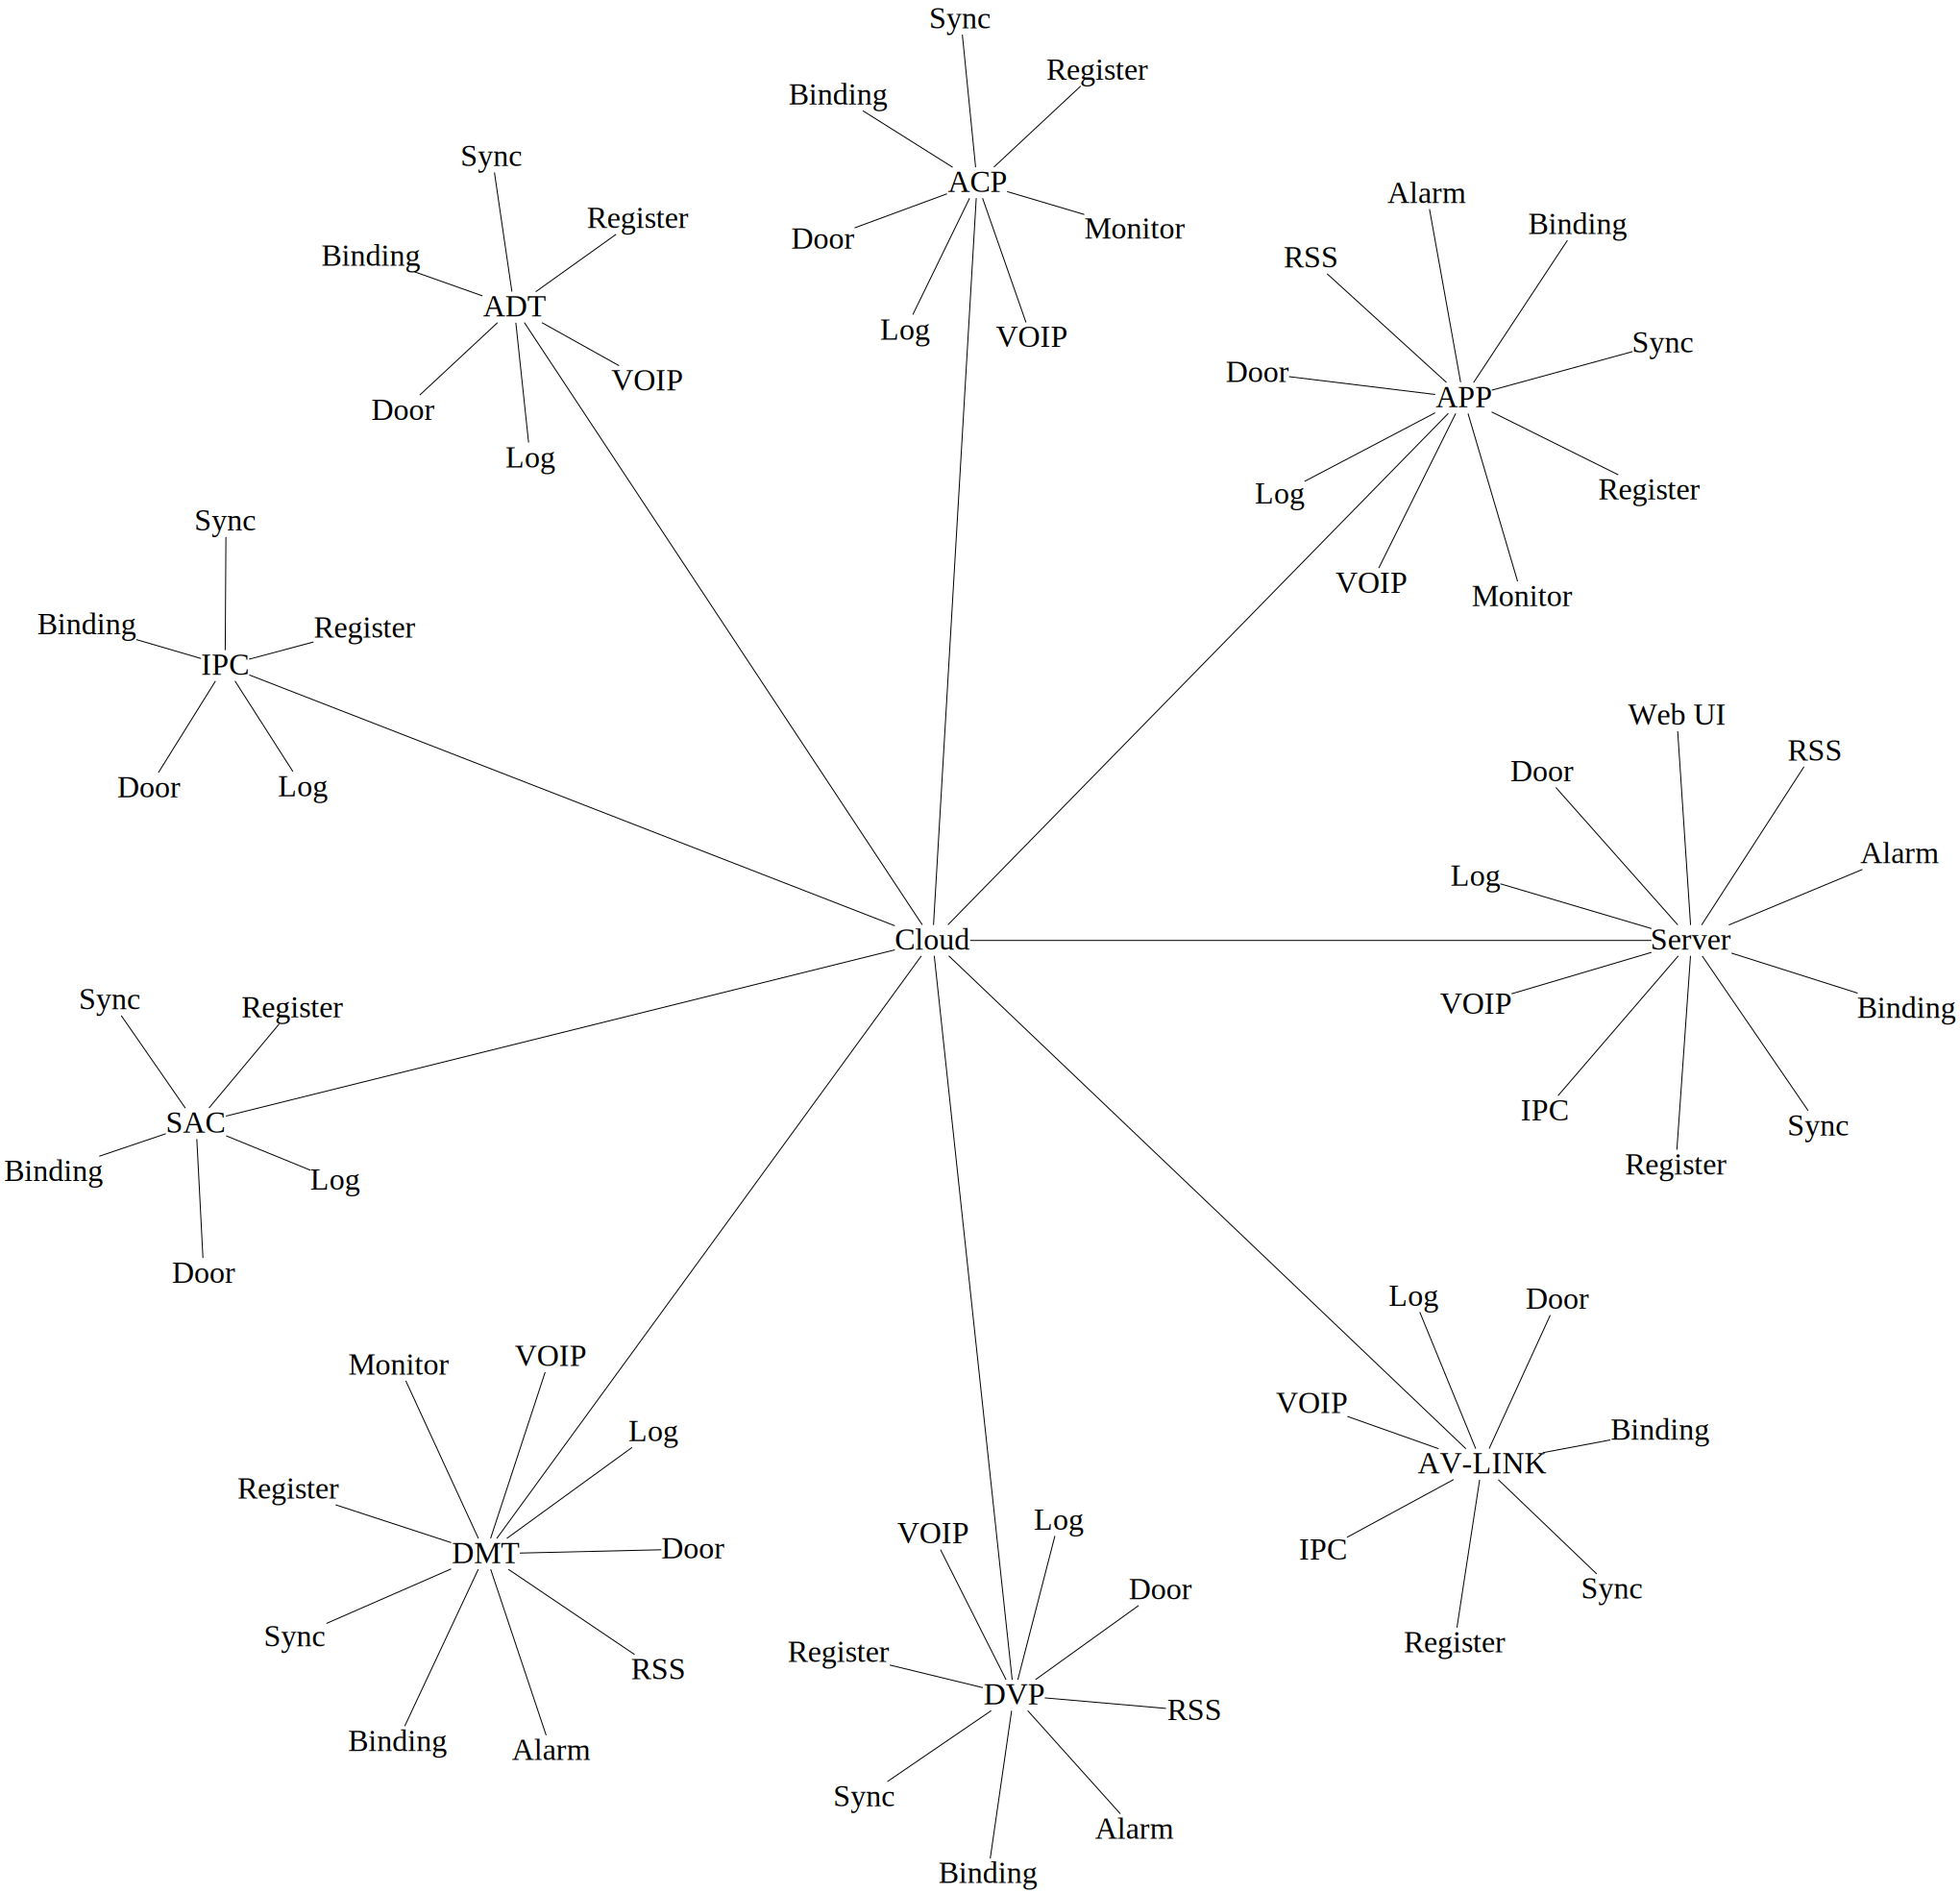
\includegraphics[width=120mm]{cloud.pdf}
    \caption{System environment.}
\end{figure}
\begin{figure}[ht]
    \centering
    \includegraphics[width=120mm]{a.eps}
    \caption{System environment.}
\end{figure}
\end{CJK}
\end{document}
